% !TEX root = ../main.tex
% chktex-file 21
\section{Hyperparameter optimization}%
\label{sec:hyperparams}

As described in the introduction, the goal of hyperparameter optimization is to find a global minimum of \(l\).
Since \(l\) is generally unknown, analytical methods or gradient descent cannot usually be applied.
The only way the get information about \(l\) is to evaluate it, which is costly.
There are multiple ways to reduce the total cost of those evaluations:
\begin{enumerate}
	\item \textbf{Number \(T\) of evaluations of \(l\):}
		During optimization multiple hyperparameter configurations \(\lambda_1, \dots, \lambda_T\) will be evaluated using \(l\).
		\(T\) is usually fixed when using a grid search or a random search.
		After evaluating \(T\) configurations, the best one is chosen.
		Those na{\"\i}ve approaches assume that \(l(\lambda)\) is independent of \(l(\lambda')\) for all pairs \(\lambda \neq \lambda'\).
		We will see that this strong assumption of independence is not necessarily true which in turn allows reducing \(T\).
	\item \textbf{Training dataset size \(S\):}
		The performance of a given configuration \(l(\lambda)\) is computed by training the learner on \(\Dtrain\) which is expensive for big datasets.
		By training on \(S\) instead of \(|\Dtrain|\) datapoints the evaluation can be sped up.
	\item \textbf{Number of training iterations \(E\):}
		Depending on the learner, training often is an iterative process, e.~g.\@ gradient descent.
		To speed up hyperparameter optimization training could be terminated before convergence.
\end{enumerate}

\subsection{FABOLAS}%
\label{sec:hyperparams:fabolas}

The first approach we will discuss is called FABOLAS (Fast Bayesian Optimization of Machine Learning Hyperparameters on Large Datasets)~\cite{Klein2016}.
It can be applied to any learner \(L\) and is based upon two main ideas:
\begin{enumerate}
	\item The validation loss \(l\) is modeled as a \textit{Gaussian process} (GP) \(f\) based on the assumption that two configurations \(\lambda_1\) and \(\lambda_2\) will perform similar if they are similar according to some kernel \(k(\lambda_1, \lambda_2)\).
		The Gaussian process \(f\) is used as a surrogate to estimate the expected value and variance of \(l\) given \(\lambda\).
		Using \textit{Bayesian optimization} \(l\) will be probed at promising positions to iteratively improve \(f\).
		Hyperparameter configurations that are expected to perform worse than the current optimum will not be probed.
		This effectively reduces \(T\).
	\item The training dataset size \(S\) is modeled as an additional hyperparameter of \(f\) giving the optimizer an additional degree of freedom.
		This allows extrapolating the value of \(l\) when trained on the complete dataset while only probing smaller subsets
		which effectively reduces \(S\).
\end{enumerate}
We will now describe how those two ideas can be applied.

\subsubsection{Gaussian processes}%
\label{sec:hyperparams:fabolas:gaussian}

A Gaussian process is a family of random variables \({(X_\theta)}_{\theta \in \Theta}\), s.~t.\@ every finite subset of them follows a multivariate normal distribution.
It is described by a prior mean function \(\mu_0(\theta) = \mathbb{E}[X_\theta]\) and a positive-definite kernel \(k(\theta_1, \theta_2) = \mathit{Cov}(X_{\theta_1}, X_{\theta_2})\).
Let \(\mathcal{D}_n = {\{(\bm{\theta}_i, \bm{y}_i)\}}_{i = 1}^{n}\) denote a set of observations.
Those observations can be used to update the means and variances of the RVs via Gaussian process regression:
\begin{align}
	\bm{m} :=&\ {(\mu_0(\bm{\theta}_1), \dots, \mu_0(\bm{\theta}_n))}^T \nonumber \\
	\bm{k}(\theta) :=&\ {(k(\bm{\theta}_1, \theta), \dots, k(\bm{\theta}_n, \theta))}^T \nonumber \\
	\bm{K} \in&\ \mathbb{R}^{n \times n}, \bm{K}_{ij} := k(\bm{\theta}_i, \bm{\theta}_j) \nonumber \\
	\mathbb{E}[X_\theta | \mathcal{D}_n] :=&\ \mu_n(\theta) = m_0(\theta) + \bm{k}{(\theta)}^T \bm{K}^{-1} (\bm{y} - \bm{m}) \\
	\mathit{Cov}(X_\theta, X_{\theta'} | \mathcal{D}_n) :=&\ k(\theta, \theta') - \bm{k}{(\theta)}^T \bm{K}^{-1} \bm{k}(\theta')
\end{align}

FABOLAS works by modeling the loss function \(l\) as a Gaussian process \(f \sim \mathcal{GP}(m, k)\) with parameter set \(\Theta := \Lambda \times [0, 1]\) where \(\mu_0(\lambda, s) = \mathbb{E}[l(\lambda)\, |\, \text{relative training set size}\ s]\).
To model the covariances between different combinations of hyperparameters and training set sizes, the following product kernel is used:
\begin{align}
	k((\lambda, s), (\lambda', s')) :=&\ k_{\nicefrac{5}{2}}(\lambda, \lambda') \cdot (\phi^T(s) \cdot \Sigma_{\phi} \cdot \phi(s')) \\
	k_{\nicefrac{5}{2}}(\lambda, \lambda') :=&\ \beta \left(1 + \sqrt{5}\, d(\lambda, \lambda') + \frac{5}{3} d^2(\lambda, \lambda')\right) e^{- \sqrt{5}\, d(\lambda, \lambda')}
\end{align}

\textit{TODO:\@ explain the kernel (Matérn kernel, Mahalanobis distance etc.)}

\subsubsection{Bayesian optimization}%
\label{sec:hyperparams:fabolas:bayesian}

To find \(\arg\min_\lambda l(\lambda)\) the bias and variance of \(f\) has to be reduced by probing \(l\) at promising positions.
This is called Bayesian optimization.
The estimated minimum after \(n\) probes is described by \(\arg\min_\lambda \mu_n(\lambda, s = 1)\), i.~e.\@ the configuration with the smallest predicted error on the full test dataset.
To reduce the number of probes required until this minimum converges, an \textit{acquisition function} is used.
Its role is to trade-off exploration vs.\@ exploitation of \(l\) by describing the expected utility of probing \((\lambda_{n+1}, s_{n+1})\) given a set of previous probes \(\mathcal{D}_n\).
FABOLAS uses an aquisition function that rates configurations by their \textit{information gain} per computation time:
\begin{align}
	a_F(\lambda, s) := \frac{1}{c(\lambda, s)} \mathbb{E}_y\Biggl[ p(y\, |\, \lambda, s, \mathcal{D}_n)\ \cdot &\int p(\hat{\lambda} \in \arg\min_{\lambda'}{l(\lambda')}\, |\, \mathcal{D}_n \cup \{(\lambda, s, y)\}) \\
	\cdot&\ \log\frac{p(\hat{\lambda} \in \arg\min_{\lambda'}{l(\lambda')}\, |\, \mathcal{D}_n \cup \{(\lambda, s, y)\})}{u(\hat{\lambda})} \mathrm{d}\hat{\lambda}\, \Biggr] \nonumber
\end{align}
\textit{TODO:\@ explain the aquisition function (Kullback-Leibler divergence, cost estimation model)}

\subsubsection{Evaluation}%
\label{sec:hyperparams:fabolas:eval}

\begin{figure}[h]
	\begin{subfigure}{0.5\textwidth}
		\centering
		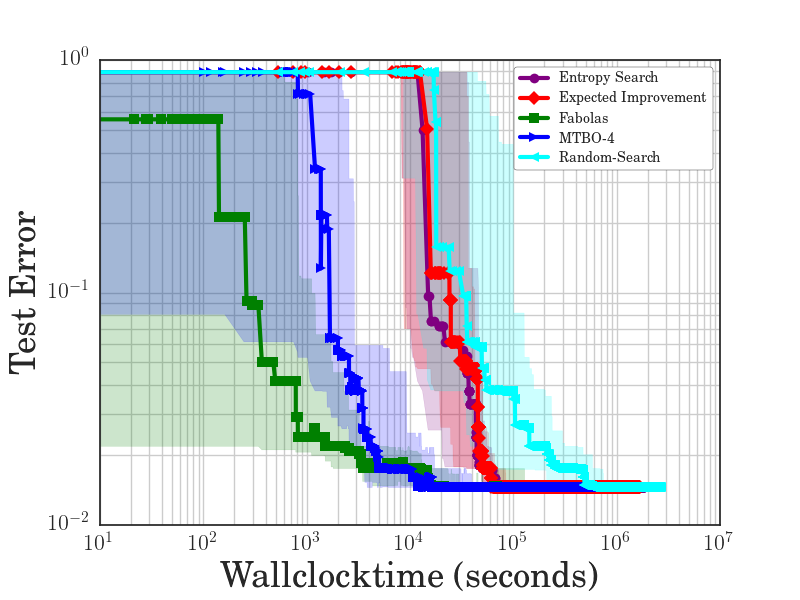
\includegraphics[width=0.85\linewidth]{gfx/fabolas/time1.png}
	\end{subfigure}
	\begin{subfigure}{0.5\textwidth}
		\centering
		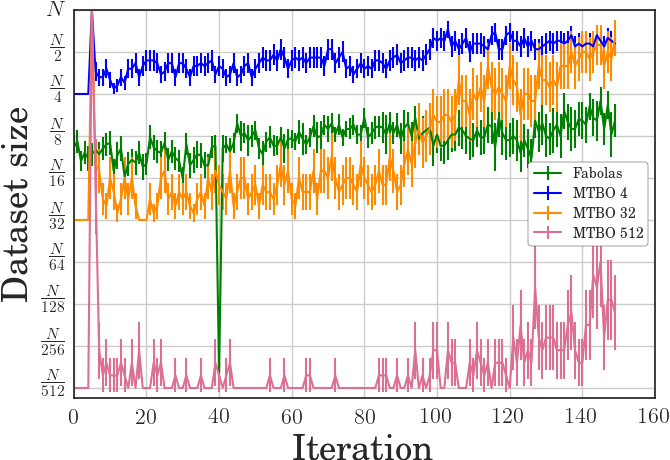
\includegraphics[width=0.95\linewidth]{gfx/fabolas/size.png}
	\end{subfigure}
	\caption{\textit{TODO}}\label{fig:fabolas}
\end{figure}

\subsection{Learning Curve Extrapolation}%
\label{sec:hyperparams:earlyterm}

The second approach for speeding up hyperparameter optimization focuses on reducing the number of training iterations \(E\).
It can in principle be applied to any iterative learner and can be integrated into any hyperparameter optimizer.
The idea is to monitor the learning curve of a learner during training with a hyperparameter configuration \(\lambda\).
If it is unlikely that a good accuracy will be reached with \(\lambda\), training will be terminated before convergence.

The method was first described by \citet{Domhan2015} in the context of hyperparameter optimization for \textit{deep neural networks} (DNNs) that are trained using stochastic gradient descent.

\textit{TODO:\@ explain the extrapolation model}
